\chapter{Phân tích yêu cầu và thiết kế hệ thống}
\label{ch:phan-tich-thiet-ke}

\section{Khảo sát bài toán}

Bài toán đặt ra là xây dựng khung kiểm soát an toàn cho ứng dụng RAG/LLM quy mô lab: chặn hoặc xử lý prompt độc hại, giảm rò rỉ qua đầu ra, kiểm soát nguồn tài liệu, và đảm bảo gói mã nguồn bàn giao không chứa artifact cấm hoặc cấu trúc không an toàn. Yêu cầu học thuật nhấn mạnh tính tái lập, fail-closed và trung thực bằng chứng thay vì tối ưu hiệu năng production.

\section{Mục tiêu của hệ thống}

\begin{enumerate}
    \item Cung cấp cổng (gateway) trung gian xử lý yêu cầu RAG/chat với các lớp guard.
    \item Cho phép so sánh baseline (không guard) và có guard trên cùng bộ test tổng hợp.
    \item Đo và so sánh hiệu quả của tường trên bộ đánh giá bảo mật tổng hợp.
    \item Ghi nhật ký quyết định guard dạng content-free, không rò rỉ nội dung nhạy cảm thô.
\end{enumerate}

\section{Phạm vi chức năng}

\textbf{Trong phạm vi:} guard rule-based và Semantic Judge; RAG demo với BM25 kết hợp embedding; Mock Provider và mô hình cục bộ ollama; bộ benchmark tấn công/lành tính tổng hợp. \textbf{Ngoài phạm vi:} fine-tune mô hình, SIEM, Kubernetes, multi-turn adversary thực chiến, và đánh giá trên LLM hay dữ liệu doanh nghiệp thật.

\section{Yêu cầu chức năng}

\subsection{Kiểm tra dữ liệu đầu vào}
Phát hiện injection/jailbreak/pattern rủi ro; trả về Allow/Block/Sanitize/Log theo thiết kế hành vi.

\subsection{Kiểm tra ngữ cảnh truy hồi}
Phát hiện chỉ thị ẩn, tài liệu mạo danh thẩm quyền và mẫu poisoning trong ngữ cảnh RAG; hỗ trợ làm sạch từng đoạn.

\subsection{Kiểm tra dữ liệu đầu ra}
Rà DLP/pattern nhạy cảm trên phản hồi; fail-closed khi vi phạm rõ.

\subsection{Kiểm soát truy cập nguồn tài liệu}
Áp kiểm soát truy cập theo vai trò/phòng ban (RBAC) trước bước truy hồi; người dùng chỉ truy hồi được tài liệu trong phạm vi quyền.

\subsection{Ghi nhận và tổng hợp kết quả}
Ghi quyết định guard dưới dạng JSON content-free với mã lý do ổn định, không lộ nội dung nhạy cảm thô.

\begin{table}[H]
\centering
\caption{Tóm tắt nhóm yêu cầu chức năng chính}
\label{tab:fr-summary}
\begin{tabular}{@{}p{0.18\linewidth}p{0.72\linewidth}@{}}
\toprule
\textbf{Mã nhóm} & \textbf{Mô tả} \\
\midrule
FR-IN  & Guard đầu vào và quyết định hành vi \\
FR-CTX & Guard ngữ cảnh truy hồi (chỉ thị ẩn, poisoning) \\
FR-OUT & Guard đầu ra / DLP \\
FR-RAG & Pipeline truy hồi + kiểm soát truy cập RBAC theo nguồn \\
FR-LOG & Nhật ký/mã lý do ổn định, content-free \\
\bottomrule
\end{tabular}
\end{table}

\section{Yêu cầu phi chức năng}

\subsection{Tính an toàn}
Fail-closed khi thiếu neo tin cậy hoặc cấu trúc không hợp lệ; không mặc định cho qua.

\subsection{Tính tái lập}
Hạt giống/fixture cố định; Mock Provider tất định; băm SHA-256 cho artifact đóng băng.

\subsection{Tính xác định}
Cùng đầu vào cho cùng cấu hình cho kết quả ổn định trong môi trường lab đã mô tả.

\subsection{Khả năng kiểm tra}
Bộ pytest cho các guard và pipeline RAG; bộ chạy đánh giá bảo mật tái lập được, có ghi provenance.

\subsection{Khả năng bảo trì}
Tách module theo từng guard và thành phần truy hồi; tránh hard-code secret.

\section{Mô hình kiến trúc tổng thể}

Kiến trúc logic gồm ba lớp: (1)~lớp ứng dụng/gateway FastAPI; (2)~chuỗi guard phòng thủ nhiều lớp; (3)~cơ chế truy hồi lai kết hợp kiểm soát truy cập RBAC và mô hình ngôn ngữ (Mock hoặc cục bộ). Mọi lớp chia sẻ nguyên tắc fail-closed và ghi nhật ký content-free.

\begin{figure}[H]
\centering
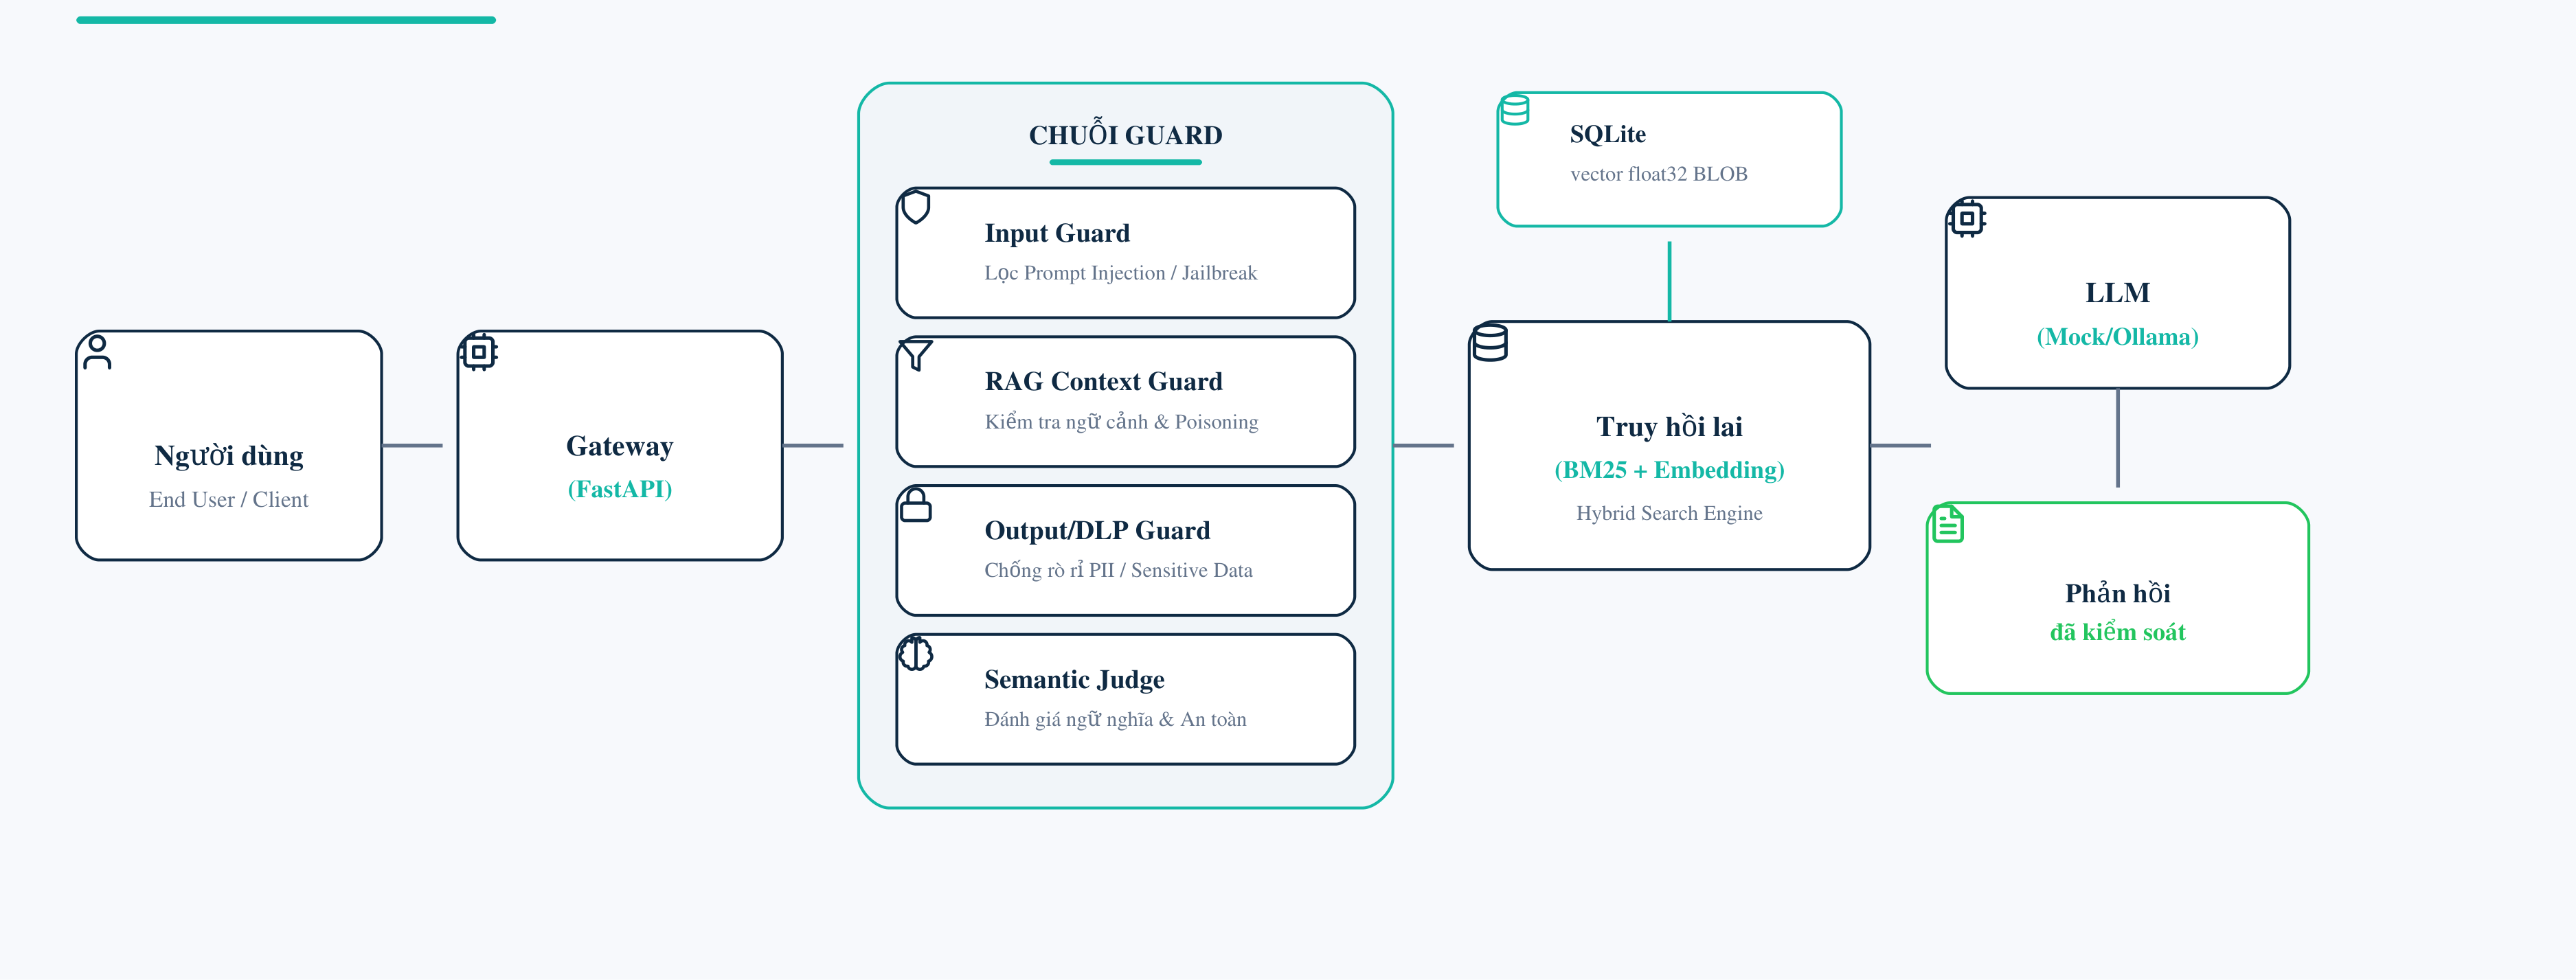
\includegraphics[width=\linewidth]{figures/fig-kien-truc.png}
\caption{Kiến trúc tổng thể hệ thống Shield AI}
\label{fig:arch-logic}
\end{figure}

Hình~\ref{fig:arch-logic} mô tả đường đi của một yêu cầu từ trái sang phải: người
dùng gửi câu hỏi tới Gateway (FastAPI), qua chuỗi guard gồm Input Guard, RAG
Context Guard, Output/DLP Guard và Semantic Judge; bước truy hồi lai (BM25 kết
hợp embedding) đọc dữ liệu từ SQLite với vector \texttt{float32} lưu dạng BLOB,
trước khi câu hỏi tới mô hình ngôn ngữ và trả về phản hồi đã được kiểm soát.

\section{Kiến trúc phòng thủ nhiều lớp của Shield AI}

Hệ thống \textbf{Enterprise LLM Security Framework (Shield AI)} áp dụng nguyên
tắc \emph{phòng thủ theo chiều sâu} (defense-in-depth): mỗi yêu cầu đi qua một
chuỗi guard độc lập, mỗi guard chặn một lớp mối đe doạ khác nhau, và một guard
thất bại vẫn còn các lớp sau. Bốn lớp guard được hiện thực như sau.

\begin{table}[H]
\centering
\caption{Bốn lớp guard phòng thủ theo chiều sâu}
\label{tab:guard-layers}
\begin{tabularx}{\linewidth}{@{}p{0.24\linewidth}p{0.20\linewidth}X@{}}
\toprule
\textbf{Lớp guard} & \textbf{Cơ chế} & \textbf{Mối đe doạ xử lý} \\
\midrule
Input Guard & Luật regex/mẫu & Prompt injection trực tiếp, jailbreak, ghi đè chỉ thị hệ thống \\
RAG Context Guard & Luật trên ngữ cảnh truy hồi & Data poisoning, chỉ thị ẩn trong tài liệu, ngữ cảnh mạo danh thẩm quyền \\
Output Guard / DLP & Mẫu bí mật + DLP + canary & Rò rỉ khoá API, thông tin nhạy cảm, PII và mã canary seed từ kho trong phản hồi \\
Semantic Judge & LLM cục bộ phán đoán & Tấn công ngữ nghĩa (đóng vai, mạo danh cấp trên) mà luật không bắt được \\
\bottomrule
\end{tabularx}
\end{table}

Ba lớp đầu là \emph{tất định} (rule-based): cùng đầu vào luôn cho cùng quyết
định, dễ giải thích và không phụ thuộc mô hình. Lớp Semantic Judge là tuỳ chọn,
dùng một mô hình ngôn ngữ cục bộ để bắt các đòn tấn công dựa trên ngữ dụng xã
hội mà mẫu regex bỏ lọt --- đánh đổi lại là chi phí tính toán và rủi ro chặn
nhầm cao hơn (phân tích định lượng ở Chương~4).

\subsection{Cơ chế truy hồi tối ưu: Vectorized Hybrid Retrieval}

Trước khi qua các guard nội dung, ngữ cảnh được truy hồi bằng cơ chế lai
(hybrid) kết hợp: (1)~xếp hạng từ khoá BM25 trên SQLite FTS5, và (2)~xếp hạng
ngữ nghĩa bằng embedding cục bộ, hợp nhất bằng Reciprocal Rank Fusion.

Điểm ngữ nghĩa được tối ưu ở hai tầng. \textbf{Về lưu trữ}, vector embedding
được lưu dưới dạng khối nhị phân \texttt{float32} chuẩn hoá sẵn (BLOB) trong
SQLite thay vì chuỗi JSON; khi truy vấn chỉ cần đọc bộ nhớ (\texttt{memcpy})
thay vì phân tích lại hàng trăm số thực. \textbf{Về tính toán}, do vector đã
chuẩn hoá đơn vị nên độ tương đồng cosine chính là tích vô hướng, và toàn bộ
kho tài liệu được chấm điểm bằng \emph{một} phép nhân ma trận (\texttt{numpy})
thay vì vòng lặp Python trên từng tài liệu.

Về mặt độ phức tạp, cải tiến này thay chuỗi $N$ vòng lặp thông dịch (mỗi vòng
$D$ phép nhân--cộng) bằng một phép nhân ma trận được thư viện BLAS tối ưu, nên
độ trễ truy hồi giảm đáng kể khi số tài liệu và số chiều tăng. % [TODO_LATENCY]: chèn số đo thực nghiệm nếu chạy benchmark; latency hiện KHÔNG báo cáo theo quyết định phương pháp L2.

\subsection{Luồng A/B chuẩn hoá: có tường vs.\ không tường}

Để đánh giá công bằng tác dụng của tường lửa, hệ thống cung cấp hai luồng chat:
\emph{có tường} (Guarded) và \emph{không tường} (Unguarded). Điểm mấu chốt bảo
đảm so sánh \emph{apples-to-apples}: cả hai luồng dùng \textbf{chung một cơ chế
truy hồi RAG và chung một ACL}, chỉ khác ở việc bật hoặc tắt chuỗi guard. Nhờ
vậy, mọi khác biệt quan sát được giữa hai luồng quy về đúng tác dụng của guard,
không lẫn với khác biệt về dữ liệu truy hồi hay phân quyền.

\begin{figure}[H]
\centering
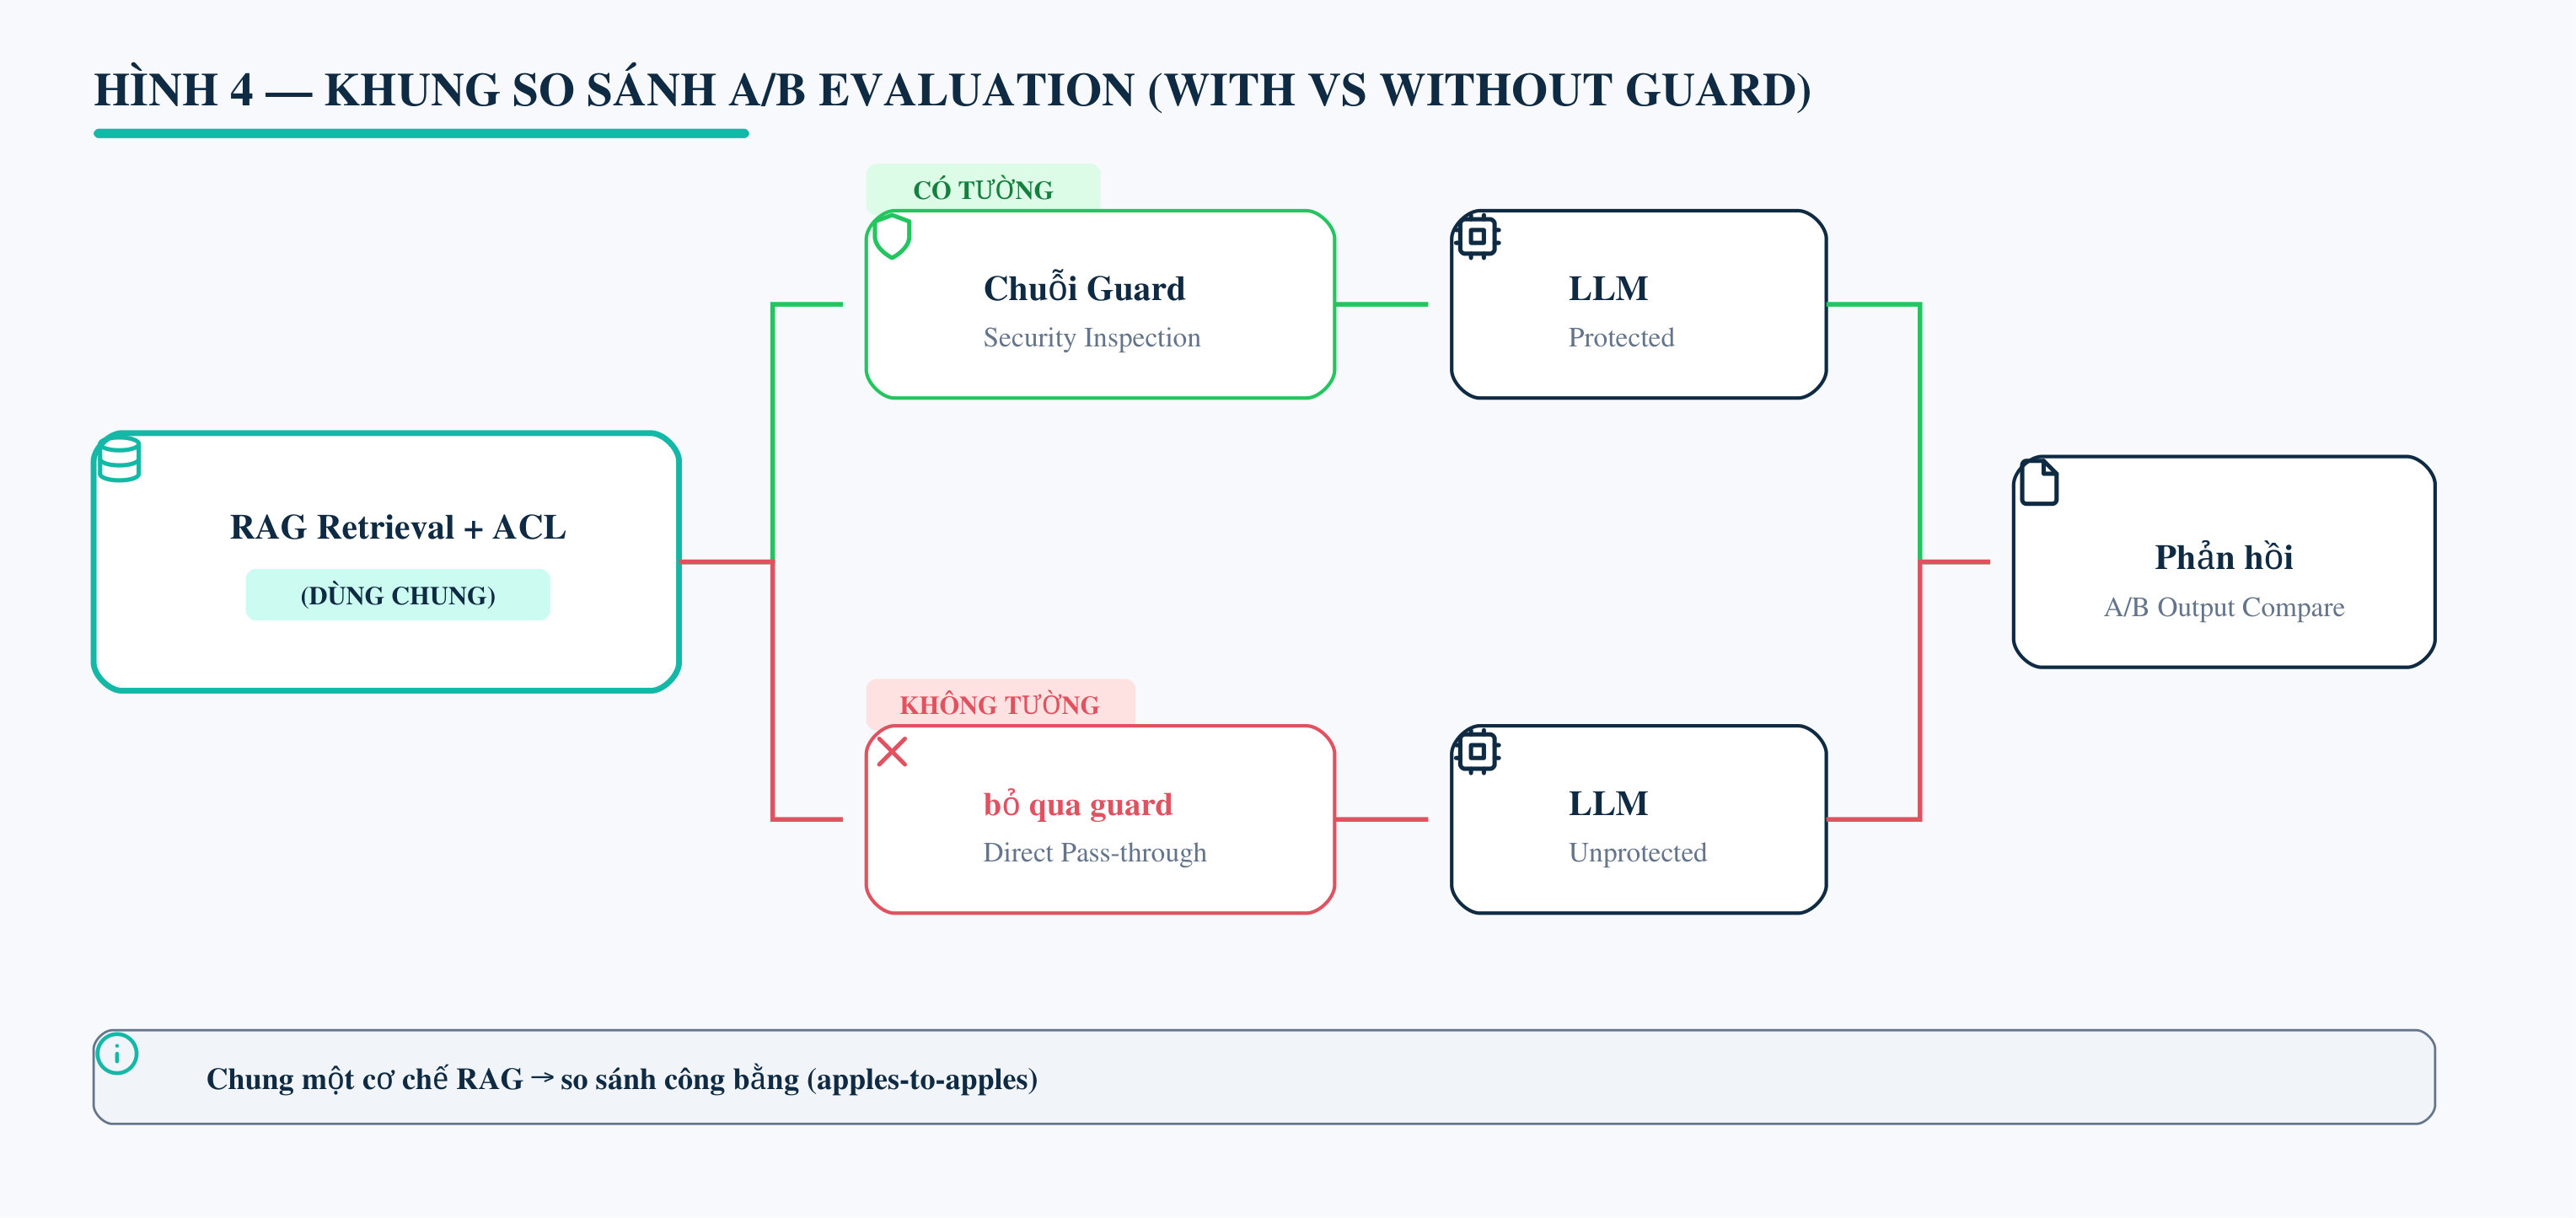
\includegraphics[width=\linewidth]{figures/fig-ab-testing.png}
\caption{Khung so sánh A/B: luồng có tường và không tường dùng chung một cơ chế RAG}
\label{fig:ab-testing}
\end{figure}

Trong Hình~\ref{fig:ab-testing}, khối \emph{RAG Retrieval + ACL} ở giữa được cả
hai luồng dùng chung: luồng ``có tường'' đi qua chuỗi guard, luồng ``không tường''
bỏ qua guard; cả hai cùng gọi một mô hình. Đây là điều kiện then chốt để so sánh
công bằng.

\section{Luồng hoạt động của hệ thống}

\begin{figure}[H]
\centering
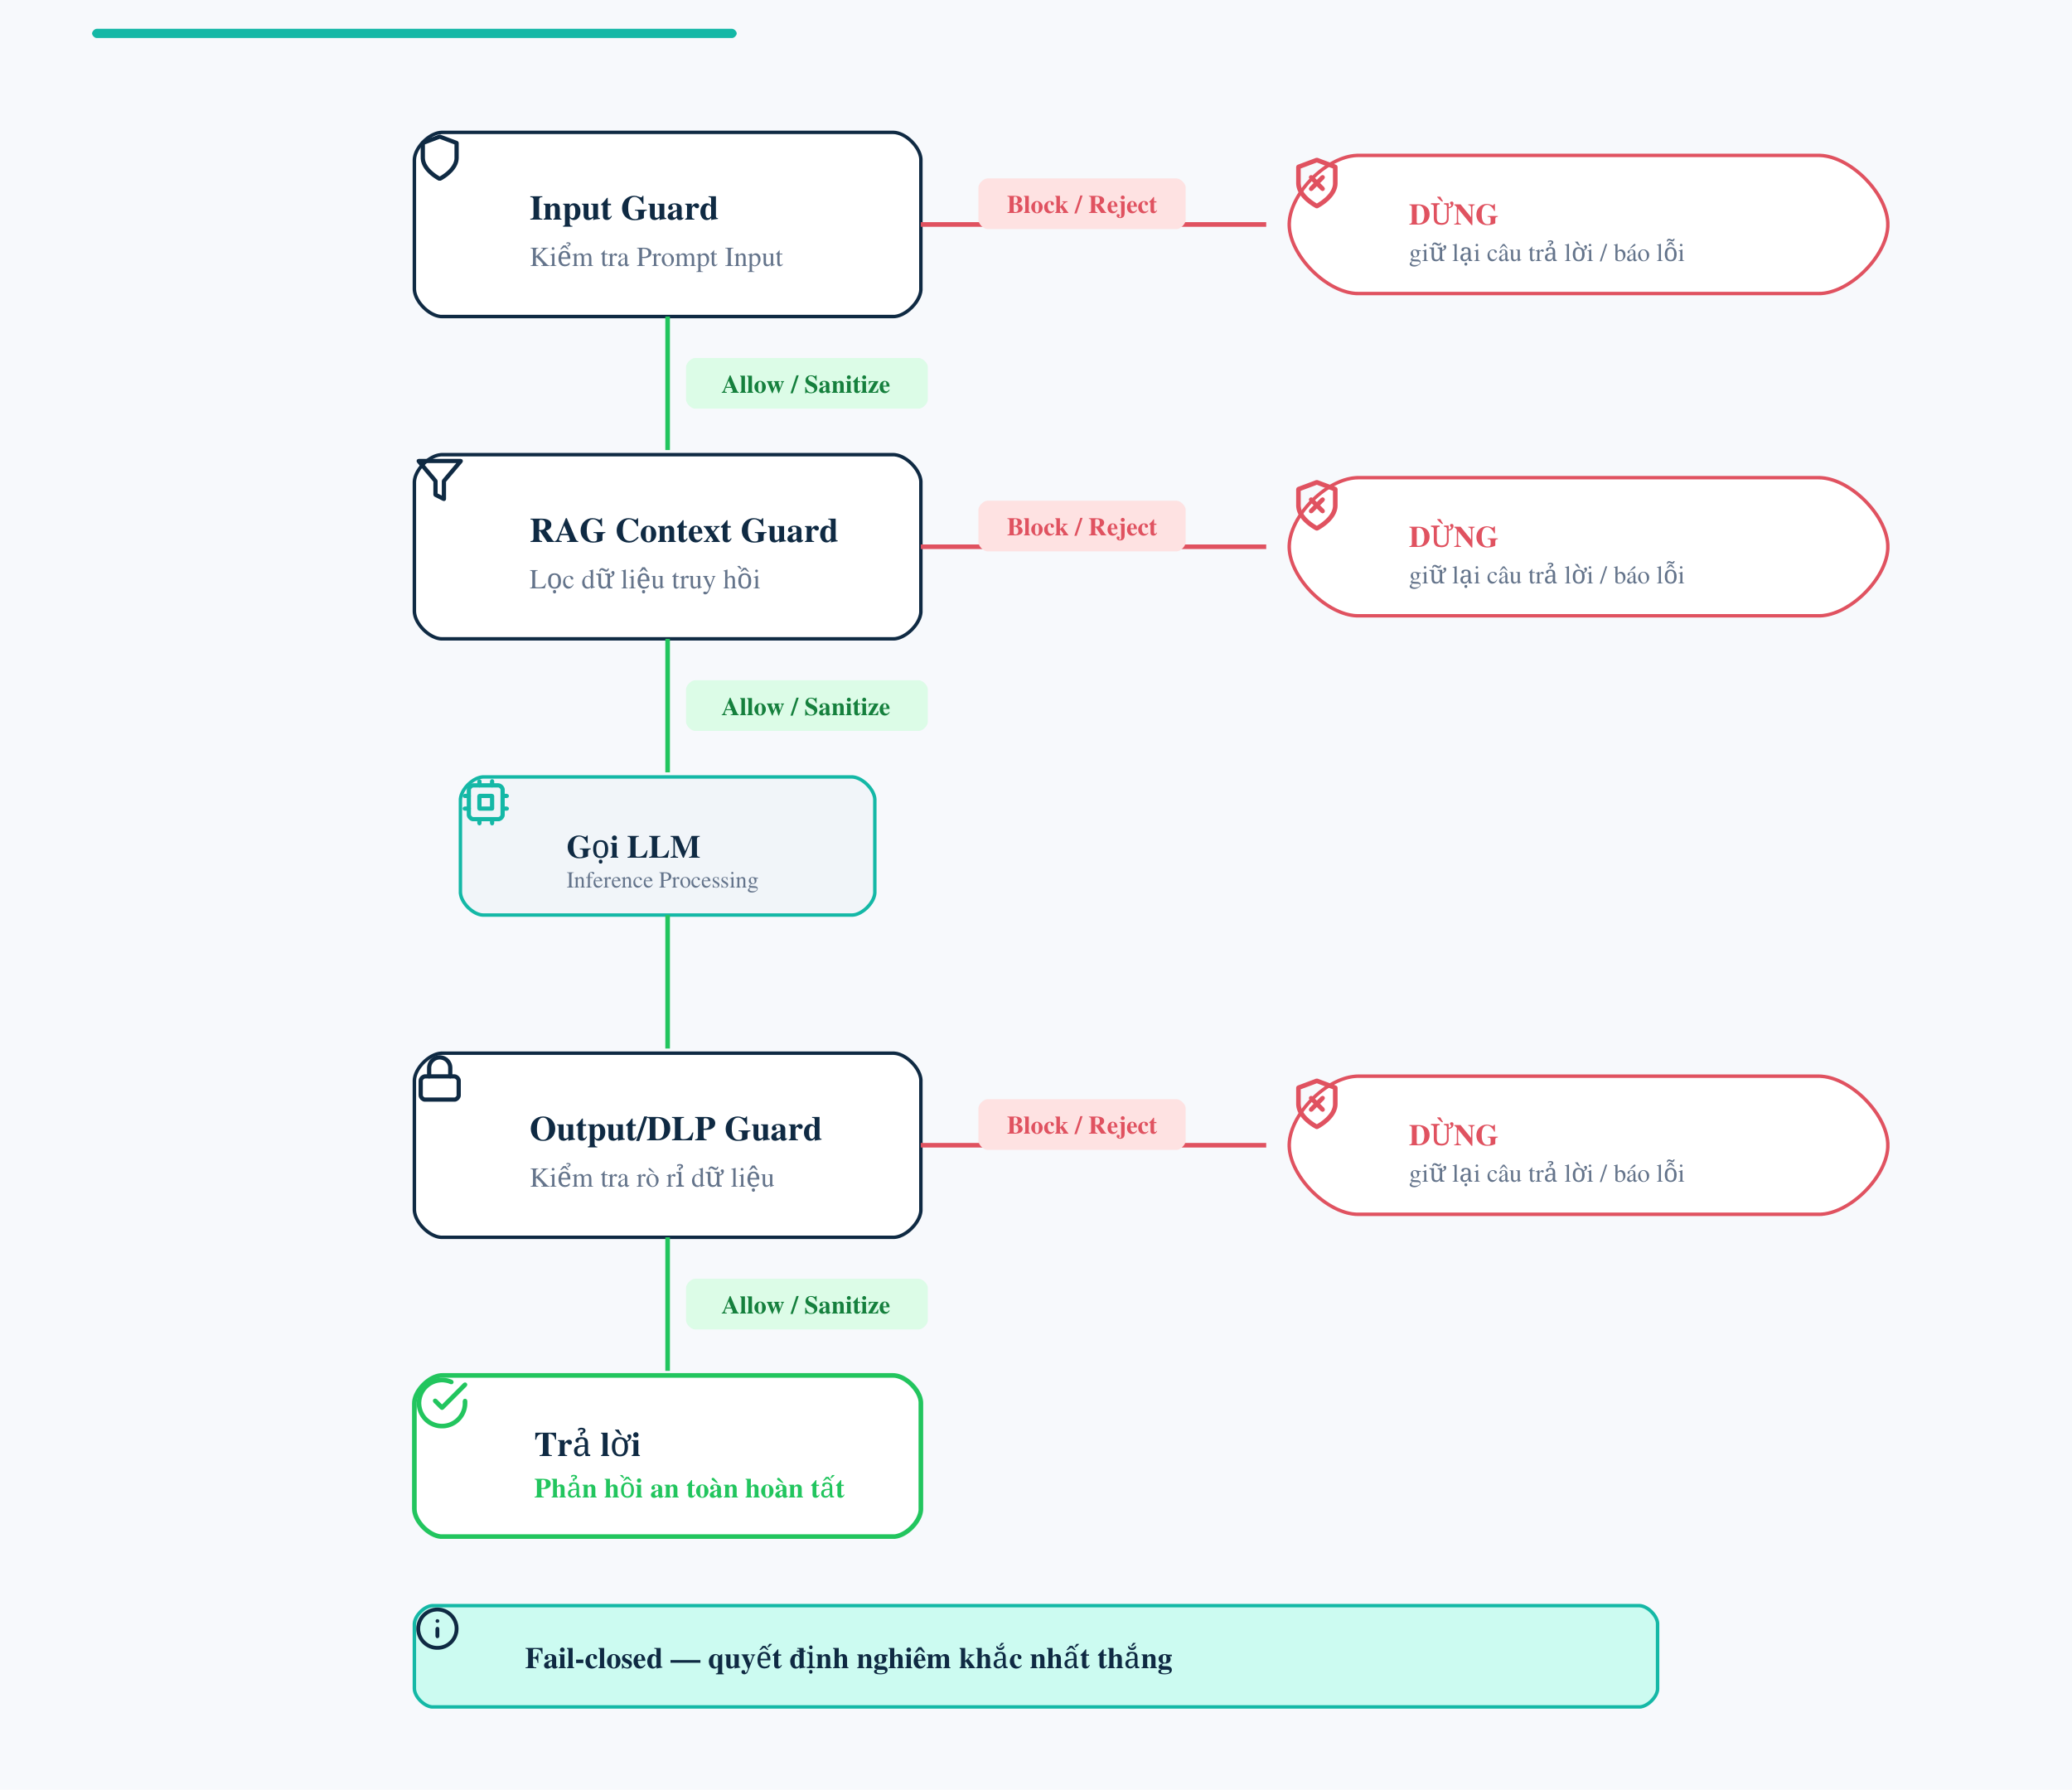
\includegraphics[width=0.85\linewidth]{figures/fig-phong-thu.png}
\caption{Chuỗi phòng thủ nhiều lớp và điểm quyết định fail-closed}
\label{fig:flow}
\end{figure}

Hình~\ref{fig:flow} thể hiện thứ tự xử lý qua các lớp guard. Tại mỗi lớp, quyết
định \emph{Block} hoặc \emph{Human-review} dừng luồng ngay và giữ lại câu trả
lời; quyết định \emph{Allow} hoặc \emph{Sanitize} cho phép đi tiếp sang lớp kế.
Nguyên tắc fail-closed bảo đảm quyết định nghiêm khắc nhất trong toàn chuỗi được
áp dụng.

\section{Thiết kế cơ chế xử lý lỗi}

Mọi lỗi trong đường xử lý được ánh xạ về quyết định an toàn: khi không chắc chắn
hoặc gặp lỗi phân tích, hệ thống fail-closed (giữ lại câu trả lời) thay vì mặc
định cho qua. Lỗi hệ thống bất ngờ được bọc ở biên công khai, không in nội dung
nhạy cảm hay traceback ra kênh công khai.

\section{Kết luận chương}

Yêu cầu và thiết kế nhấn mạnh phòng thủ nhiều lớp, fail-closed, kiểm soát truy
cập theo nguồn và tính tái lập. Chương~3 trình bày cách các thành phần được hiện
thực.
